\section{Day 17: Uniform Continuity... and with great pain, Intro to Algebraic Topology (Nov. 5, 2024)}
Outfit of the day: looks like a valorant skin i forgot which one
\begin{figure}[h]
    \centering
    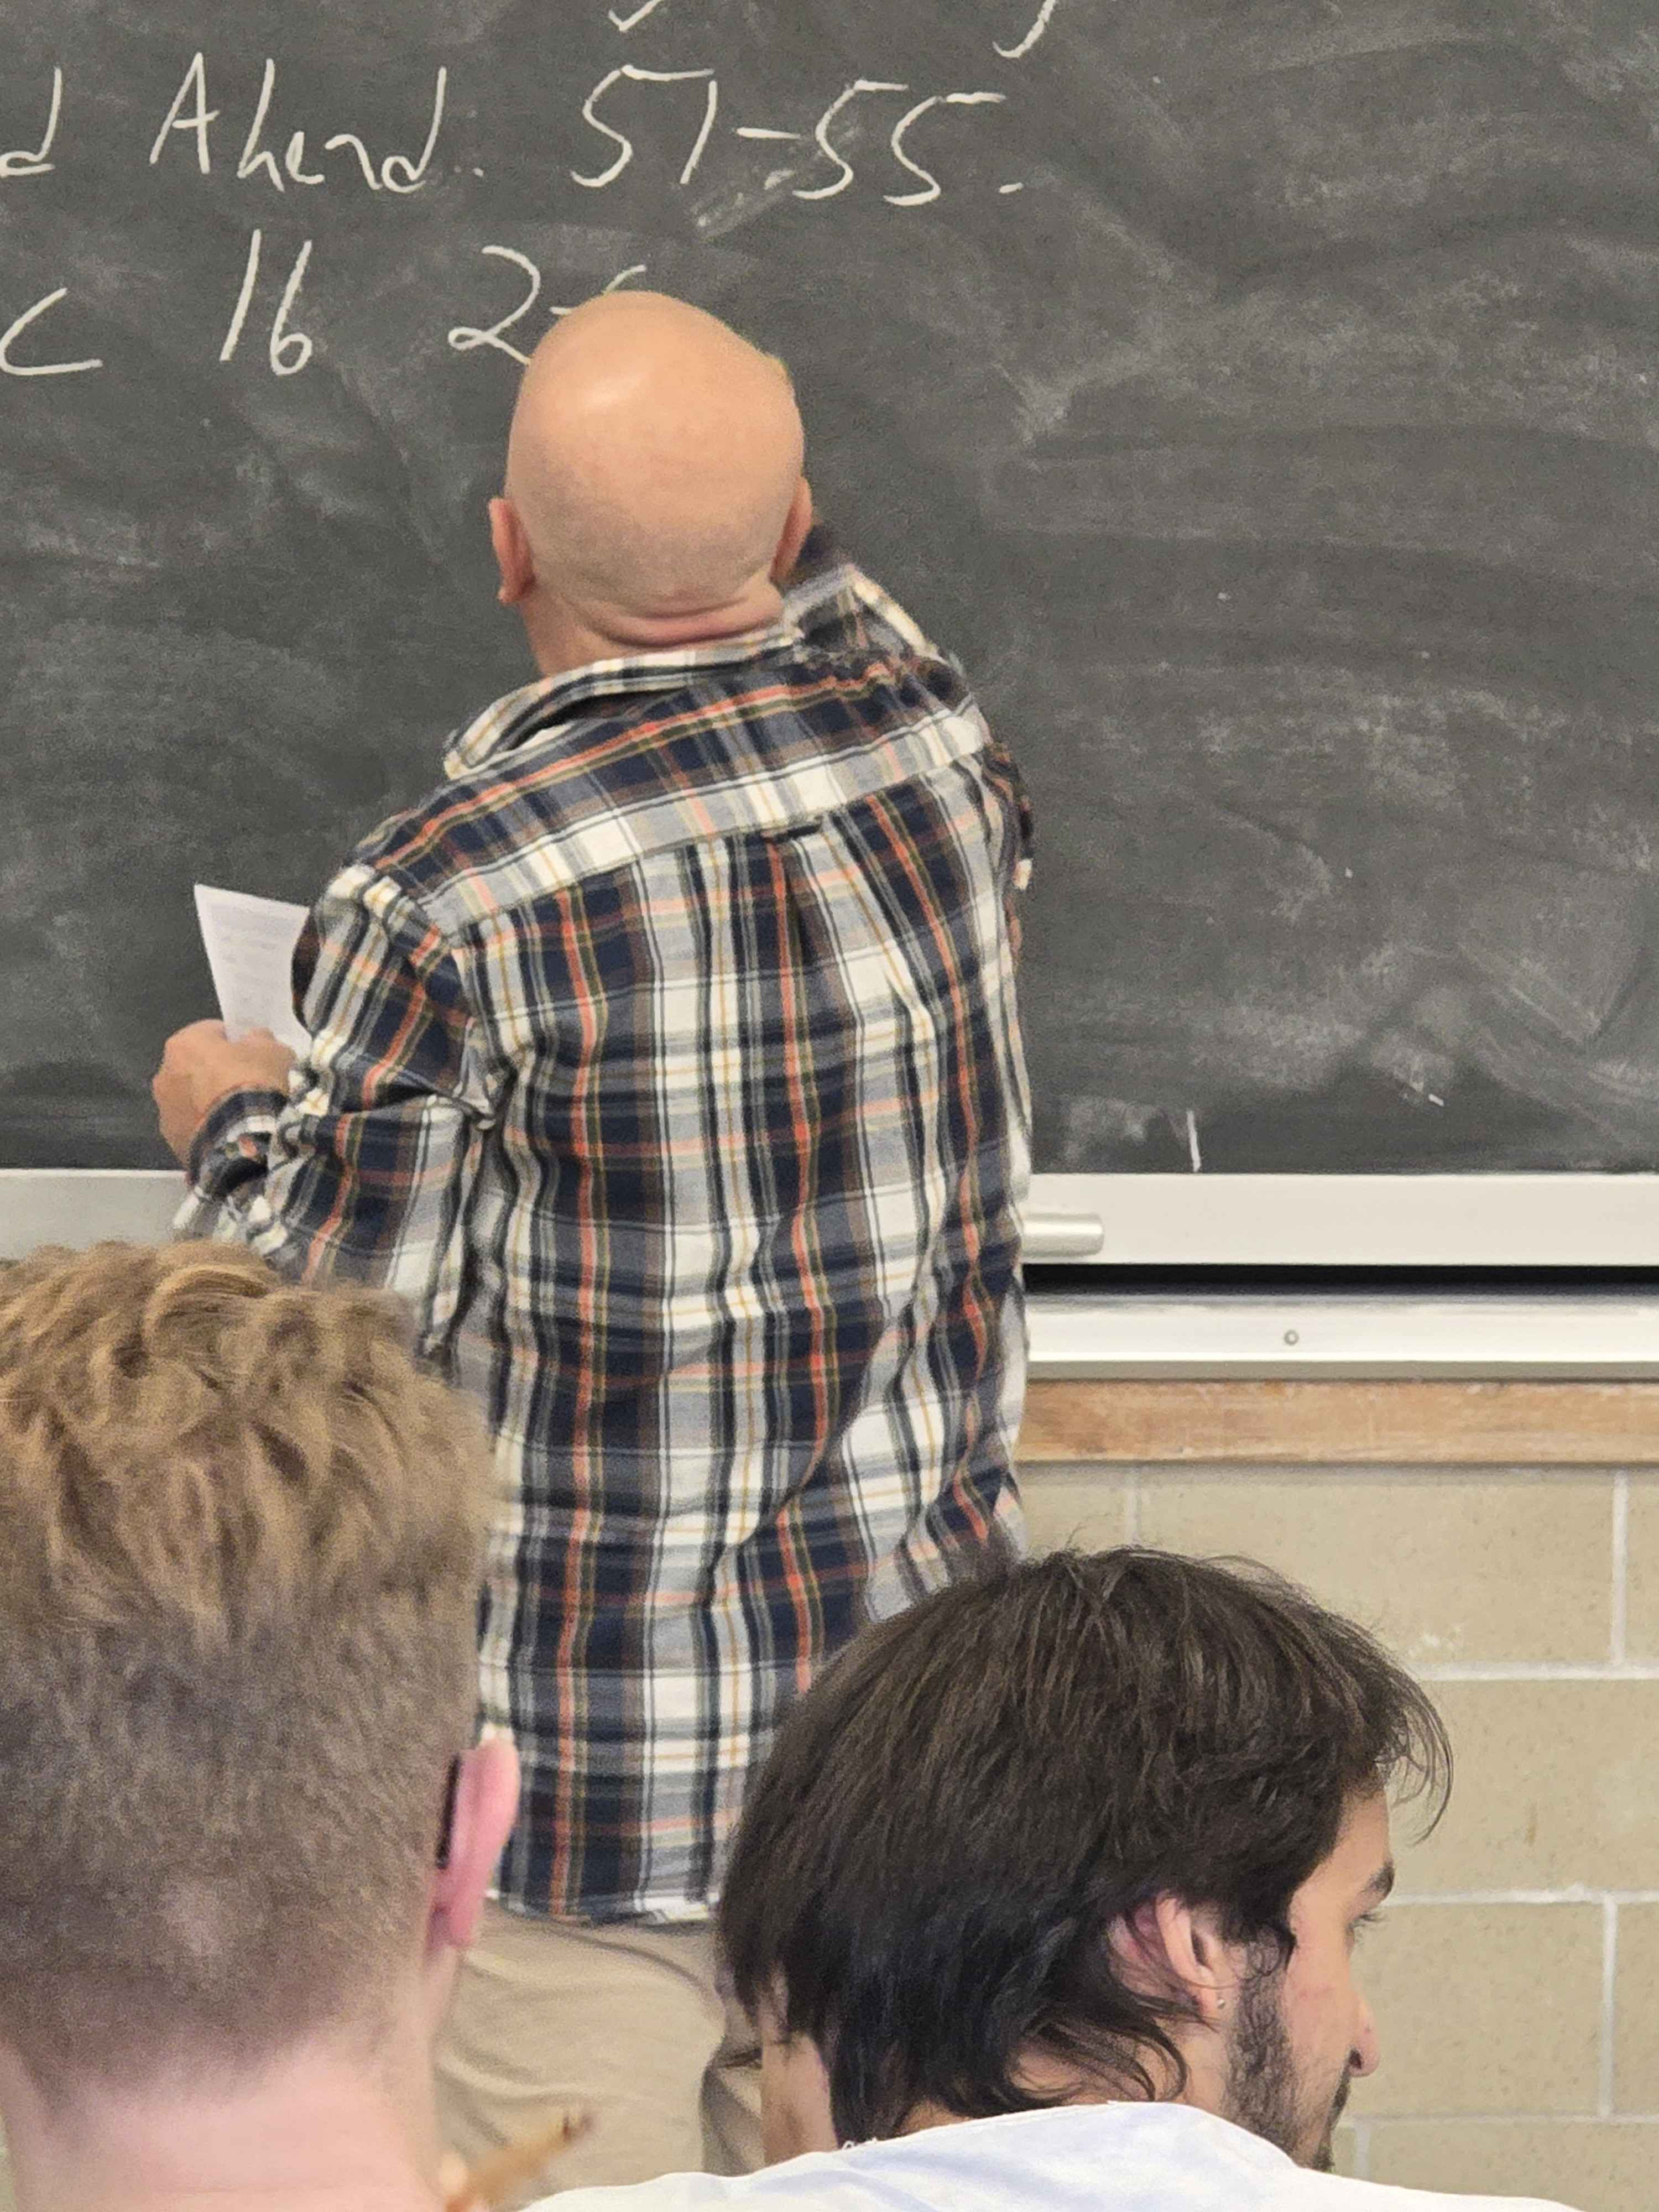
\includegraphics[scale=0.1]{MAT327 Notes/Dror Shirts/dror day 17 shirt.jpg}
\end{figure}

\noindent Read sections 26-27, and read ahead on sections 51-55 in Chapter 9. Recall that compactness is the property that every open cover admits a finite subcover. Recall that the definition of uniform continuity is given as follows; if $f : X \to Y$ is uniformly continuous, where $X, Y$ are both metric spaces; then $d_X(x_1, x_2) < \delta \implies d_Y(f(x_1), f(x_2)) < \eps$.
\begin{simplethm}
    If $X$ is compact, then any continuous function from $X$ is uniformly continuous as well.
\end{simplethm}
\noindent To prove this, we start with a lemma.
\begin{simplelemma}[Lebesgue Number Lemma]
    If $X$ is a compact metric space and $\SO$ is an open cover of $X$, then there exists some $\eps > 0$ such that for every $x \in X$, there exists $U \in \SO$ such that $B_\eps(x) \in U$.
\end{simplelemma}
\noindent Define the following function,
\[ \Delta(x) = \sup \{\delta \leq 1 \mid \exists U \in \SO \text{ s.t. } B_\delta(x) \subset U\}, \]
of which we note that the set we are taking the supremum of is necessarily nonempty since $x$ is in some open set in $\SO$, and since the set is bounded above by $1$, the supremum exists. For $y$ satisfying $d(x, y) < \eps$, we have $\Delta(y) \geq \Delta(x) - \eps$. By symmetry, we also have that $\Delta(x) \geq \Delta(y) - \eps$. This means $\abs{\Delta(x) - \Delta(y)} < \eps$, yielding that $\Delta$ is a continuous function.
\medskip\newline
Let $\delta_0 = \min_{x \in X} \Delta(x) > 0$. For $x \in X$, we have $\Delta(x) > \delta_0$, and so there exists $U \in \SO$ such that we may pick $\delta = \frac{\delta_0}{2}$ to see $B_\delta(x) \subset U$, and we are done. We call $\delta$ the \textit{Lebesgue number} of $\SO$. \footnote{i think the wikipedia proof is better... \href{https://en.wikipedia.org/wiki/Lebesgue\%27s_number_lemma}{here}} \qed
\medskip\newline
We now prove the theorem. Let $\eps > 0$ be given; by continuity, for every $x \in X$, find $\delta_x$ such that if $y \in B_{\delta_x}(x)$, then $d_Y(f(x), f(y)) < \frac{\eps}{2}$. The collection $\{B_{\delta_x}(x) \mid x \in X\}$ is an open cover of $X$, so it has a Lebesgue number $\delta > 0$ as per our lemma. Now, if $d_X(x_1, x_2) < \delta$,then $x_2 \in B_\delta(x_1)$, so there exists some $x \in X$ such that $x_1, x_2 \in B_\delta(x_1) \subset B_{\delta_x}(x)$, so
\[ d_Y(f(x_1), f(x_2)) \leq d_Y(f(x_1), f(x)) + d_Y(f(x), f(x_2)) < \frac{\eps}{2} + \frac{\eps}{2} = \eps. \qed \]

\begin{simplethm}[Tychonoff's Theorem]
    An arbitrary product of compact spaces is compact.
\end{simplethm}
\noindent This won't be proven in class, but the Axiom of Choice is used \sout{so it's a fuckin' lie}. A whole other slew of stuff also won't be covered in class pwp... here's the \href{https://drorbn.net/AcademicPensieve/Classes/24-327-Topology/WhatWeMiss.png}{list}!
\medskip\newline
\noindent We now go onto algebraic topology. Notice that in MAT327, we study topological spaces and continuous maps; in MAT240, we studied vector spaces and linear maps; set theory deals with sets and functions, and MAT347 deals with groups and homomorphisms. On Thursday, we will construct a functor $\pi_1$ from topological spaces to groups and continuous maps to homomorphisms.